\section{Analytic Geometry}
\label{sec:analyticGeo}

I will use the convention from~\cite{Buss2003}.
We use lower case names in normal font to represent scalars: $s$, $t$, $v$.
Bolt font with lower case names to represent vectors: $\mathbf{a}$, $\mathbf{b}$, $\mathbf{p}$.
Upper case names in bold face to represent set of points in the space: $\mathbf{L}$, $\mathbf{R}$ (like lines or rays).
Finally, upper case names in normal font to represent matrices: $P$, $V$, $M$.

The vectors are column vectors. In other words:
$$ \mathbf{v} = \begin{bmatrix}
  x \\ 
  y \\
  z
 \end{bmatrix} $$

Then we can use syntax like: $A \mathbf{x} = \mathbf{b}$.
To make the reading easier, in case I will need to specify a vector inside a paragraph I will use $\mathbf{v} = \langle x, y, z \rangle$

In the notation, we do not make any distinction between vectors and points, therefore the text always gives context to clarify this. 

\subsection{Line, ray and segment}
\label{sec:linedef}

In most CG applications, we use two \emph{different} points; let's call them $\mathbf{a}$ and $\mathbf{b}$ (with $\mathbf{a} \neq \mathbf{b}$) to specify a line: $\mathbf{L}$. 

However, in analytic geometry we prefer a parametric equation for the line: $\mathbf{L}(t)$.
We use a point $\mathbf{p}$, a directional vector $\mathbf{v}$ and a scalar $t$ as parameter : $\mathbf{L}(t) = \mathbf{p} + t \mathbf{v}$, with $t \in (-\infty, \infty)$.

To transform between this two representations we do: $\mathbf{v} = \mathbf{b} -\mathbf{a}$. And, then the line is: 

\begin{equation}
\mathbf{L}(s) = \mathbf{a} + s (\mathbf{b} -\mathbf{a}) = \mathbf{a} + s \mathbf{v} 
\label{eq:line}
\end{equation}
, with $s \in (-\infty, \infty)$. 

Note that the order of $\mathbf{a}$ and $\mathbf{b}$ is relevent, because of the way we define $\mathbf{v}$: it points from $\mathbf{a}$ to $\mathbf{b}$.
Also note that $\mathbf{v}$ is not necesarlly a unit vector. 

\begin{figure}[htb]
  \centering
  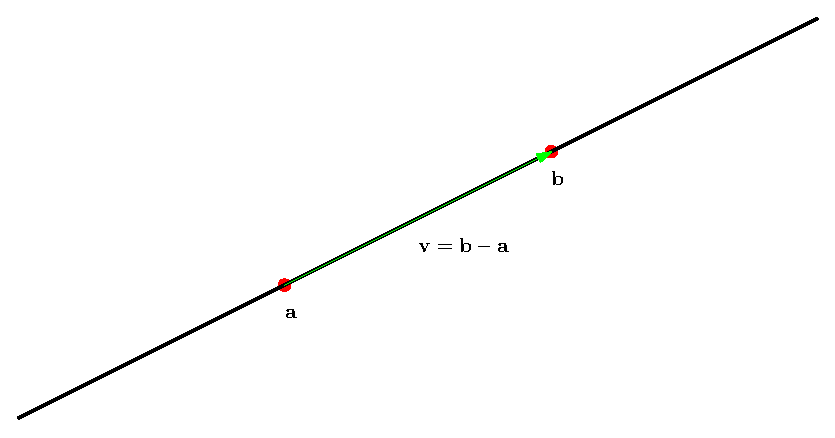
\includegraphics[width=0.85\textwidth]{img/line}
  \caption{Line identified by two points. See Equation~\ref{eq:line} }
  \label{fig:line}
\end{figure}

The Figure~\ref{fig:line} shows the line from Equation~\ref{eq:line} (in black) indentified by the points $\mathbf{a}$ and $\mathbf{b}$ (in red) and the directional vector $\mathbf{v}$ (in green).
Remember that vectors are free on the space, in this sense we can represent $\mathbf{v}$ in any place of the plane as long as we do not change his orientation (the angles it makes against the frame of reference).


On these conditions; we can give continuos values to the parameter $s$ in the Equation~\ref{eq:line}, to obtain points on the line $\mathbf{L}$.
Particulary, if we let $s = 0$ we get the point $\mathbf{a}$ and if we let $s = 1$ we get  
$\mathbf{b}$.
Moreover, any value $0 \leq s \leq 1$ will get us a point $\mathbf{p}$ inside the line segment $\overline{\mathbf{a} \mathbf{b}}$.
Any value $s > 1$ will get a $\mathbf{p} \in \mathbf{L}$, $\mathbf{p} \notin \overline{\mathbf{a} \mathbf{b}}$ that is closer to $\mathbf{b}$ than it is to $\mathbf{a}$.
Conversely, any $s < 0$ will get a $\mathbf{p} \in \mathbf{L}$, $\mathbf{p} \notin \overline{\mathbf{a} \mathbf{b}}$ that is closer to $\mathbf{a}$ than it is to $\mathbf{b}$.

We can use this last observations to identify segments and rays.
A \emph{ray} from $\mathbf{a}$ in the direction of $\mathbf{b}$ is the one that has Equation~\ref{eq:line}, with the constrain that the parameter must be $s \geq 0$.
The line \emph{segment} from $\mathbf{a}$ to $\mathbf{b}$, denoted by $\overline{\mathbf{a} \mathbf{b}}$, is the one that also follows Equation~\ref{eq:line}, with the constrain that   $0 \leq s \leq 1$.

\subsection{Point to line distance}
\label{sec:point2line}

Given a line $\mathbf{L}$ and a point $\mathbf{p}$, we want to identify the distance $d$ from $\mathbf{p}$ to $\mathbf{L}$.
It's clear that if $\mathbf{p} \in \mathbf{L}$, then $d = 0$.
Now, if $\mathbf{p} \notin \mathbf{L}$, we want the distant between $\mathbf{p}$ and a certain point $\mathbf{q}$, such that $\mathbf{q} \in \mathbf{L}$ and $d(\mathbf{q}, \mathbf{p})$ is the minimal to all other points in $\mathbf{L}$.

\begin{figure}[htb]
  \centering
  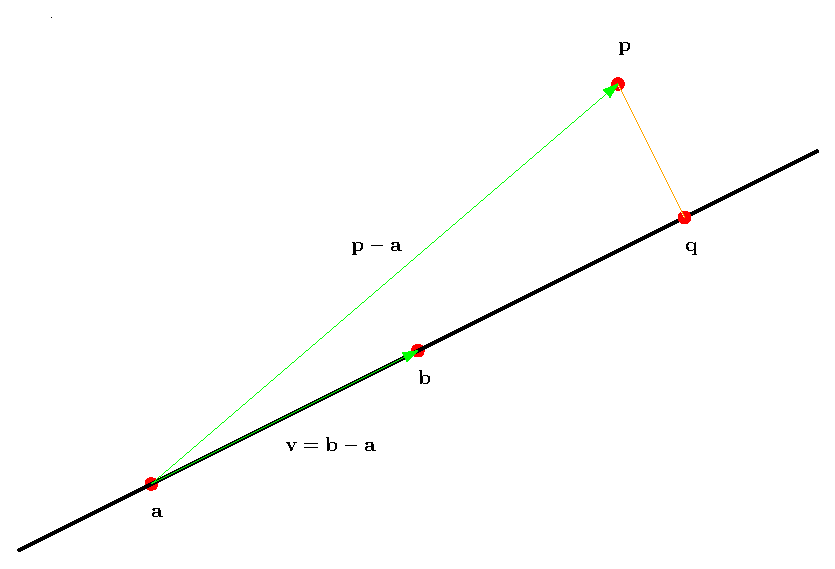
\includegraphics[width=0.85\textwidth]{img/line2point}
  \caption{Line identified by two points. See Equation~\ref{eq:line} }
  \label{fig:point2line}
\end{figure}

In other words we want the minimal distance from $\mathbf{p}$ to $\mathbf{L}$.
The Figure~\ref{fig:point2line} depicts this situation.
If we start sliding a point on $\mathbf{L}$ (starting lets say at $\mathbf{a}$) and evaluating the distance beween that point and $\mathbf{p}$, we can see that the distance begins getting smaller as we come close to $\mathbf{p}$, get his minimal value when we are right bellow $\mathbf{p}$ and then increases again. 
Indeed, the distance we are looking is between $\mathbf{p}$ and the point $\mathbf{q}$ that is in the intesection between the line $\mathbf{L}$ and the segment $\overline{\mathbf{p} \mathbf{q}}$ which is perpendicular to $\mathbf{L}$.
In the Figure~\ref{fig:point2line}, $\overline{\mathbf{p} \mathbf{q}}$ is the orange dashed line and the desired $d$ it's of course his lenght.

Before we proced; I put a quick reminder of the formula to calculate the projection of a vector $\mathbf{x}$ into another vector $\mathbf{y}$. 

\begin{equation}
\proj_{\mathbf{y}}\mathbf{x} = \dfrac{(\mathbf{x} \cdot \mathbf{y})}{|\mathbf{y}|} \dfrac{\mathbf{y}}{|\mathbf{y}|} = \dfrac{(\mathbf{x} \cdot \mathbf{y})}{|\mathbf{y}|^2}\mathbf{y}
\label{eq:proj}
\end{equation}

The Figure~\ref{fig:projection} shows this situation.
The result of $\proj_{\mathbf{y}}\mathbf{x}$ is another vector (in green in the Figure~\ref{fig:projection}) which has the same direction as $\mathbf{y}$ and whose lenght is the one that will have the shadow of $\mathbf{x}$ when its perpendiculary projected into $\mathbf{y}$.
The Equation~\ref{eq:proj} puts in evidence that $\mathbf{y}$ is a directional vector and that $\frac{(\mathbf{x} \cdot \mathbf{y})}{|\mathbf{y}|^2}$ it's his scaling lenght in units of $\mathbf{y}$.

\begin{figure}[htb]
  \centering
  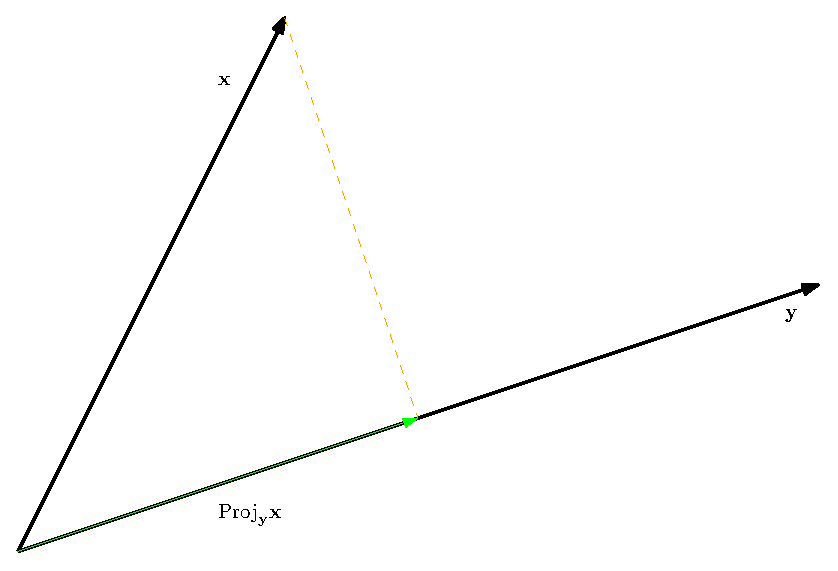
\includegraphics[width=0.60\textwidth]{img/projection}
  \caption{Projection of a vector $\mathbf{x}$ into another vector $\mathbf{y}$. See Equation~\ref{fig:projection}}
  \label{fig:projection}
\end{figure}

In order to calculate the distance, we use the scaling lenght from Equation~\ref{eq:proj} to find the corresponding parametric value $s_q$ for $\mathbf{q}$ on $\mathbf{L}$: 
\begin{equation}
s_q = \dfrac{(\mathbf{p} - \mathbf{a}) \cdot (\mathbf{b} - \mathbf{a})}{|\mathbf{b} - \mathbf{a}|^2}
\label{eq:scalarq}
\end{equation}
Then the point is:
\begin{equation}
\mathbf{q} = \mathbf{a} + s_q (\mathbf{b} -\mathbf{a})
\label{eq:pointq}
\end{equation}
And finally, the distance is $d(\mathbf{p}, \mathbf{L}) = d(\mathbf{p}, \mathbf{q})$.

\subsubsection{Point to segment distance}
\label{sec:point2segment}
A common derived problem of the previos one, is to find the distance of a point $\mathbf{p}$ to a segment $\overline{\mathbf{a}\mathbf{b}}$.
See Figure~\ref{fig:seg2point}, we see that the distance of different points depend on how are they placed with respect of the segment.
For the point $\mathbf{p}_1$ the distance to $\overline{\mathbf{a}\mathbf{b}}$ is the distance $d(\mathbf{p}_1, \mathbf{a})$, for the point $\mathbf{p}_2$ the distance is $d(\mathbf{p}_2, \mathbf{b})$ and for the point $\mathbf{p}_3$ the distance is actually the distance $d(\mathbf{p}_3, \mathbf{L})$ where $\mathbf{L}$ is the line defined by $\mathbf{a}$ and $\mathbf{b}$.

\begin{figure}[htb]
  \centering
  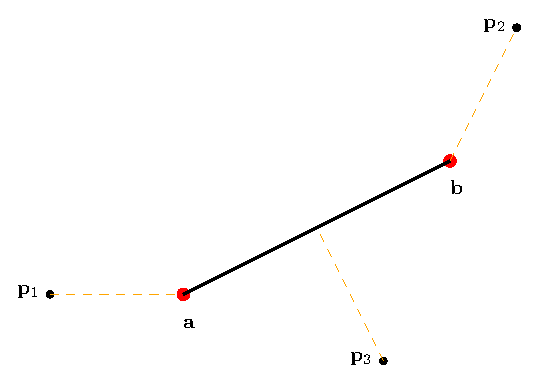
\includegraphics[width=0.50\textwidth]{img/segment2point}
  \caption{Diferents points $\mathbf{p}_i$ and their distances to segment $\overline{\mathbf{a}\mathbf{b}}$}
  \label{fig:seg2point}
\end{figure}

The observations at the end of Section~\ref{sec:linedef} and Section~\ref{sec:point2line} give us a nice Algorithm to find this distance.

{\centering
\begin{minipage}{\linewidth}
  \begin{algorithm}[H]
    \caption{Distance between a point $\mathbf{p}$ and a line segment $\overline{\mathbf{a}\mathbf{b})}$}
    \label{alg:poin2seg}
    \begin{algorithmic}[1] % The number tells where the line numbering should start 0 for no number
      \Procedure{DistancePoint2Segment}{$\mathbf{a},\mathbf{b},\mathbf{p}$} \Comment{$\mathbf{a}$, $\mathbf{b}$ and $\mathbf{p}$ are all points of the same dimension}
        \If{$\mathbf{a} = \mathbf{b}$} \Comment{There is no line, the segment it's just a point}
          \State \textbf{return} $d(\mathbf{a},\mathbf{p})$
        \EndIf
        \State $s \gets \frac{(\mathbf{p} - \mathbf{a}) \cdot (\mathbf{b} - \mathbf{a})}{|\mathbf{b} - \mathbf{a}|^2}$ \Comment{Use Equation~\ref{eq:scalarq} to get parametric value of $\mathbf{q}$}
        \If{$s < 0$} \Comment{$\mathbf{p}$ is closer to $\mathbf{a}$ than to $\overline{\mathbf{a}\mathbf{b}}$}
          \State $r \gets d(\mathbf{a},\mathbf{p})$
         \ElsIf{$s > 1$} \Comment{$\mathbf{p}$ is closer to $\mathbf{b}$ than to $\overline{\mathbf{a}\mathbf{b}}$}
          \State $r \gets d(\mathbf{b},\mathbf{p})$
        \Else \Comment{$\mathbf{p}$ is over $\overline{\mathbf{a}\mathbf{b}}$}
          \State $\mathbf{q} \gets \mathbf{a} + s (\mathbf{b} - \mathbf{a})$ \Comment{Calculate $\mathbf{q}$}
          \State $r \gets d(\mathbf{q},\mathbf{p})$
        \EndIf
        \State \textbf{return} $r$ \Comment{Distance is stored in $r$}
      \EndProcedure
    \end{algorithmic}
  \end{algorithm}
\end{minipage}
\par
}

We can have a less clear, but a little bit more efficient algorithm.
The branching due the value of $s$ can be reduced if we use a clamp (by the means of $\Max$ and $\Min$ functions).
The Algorthm~\ref{alg:poin2seg2} shows this idea and Listing~\ref{lst:poin2seg2} shows the implementation in C++ using the \href{https://glm.g-truc.net}{GLM} library.

{\centering
\begin{minipage}{\linewidth}
  \begin{algorithm}[H]
    \caption{Distance between a point $\mathbf{p}$ and a line segment $\overline{\mathbf{a}\mathbf{b})}$  (Second version)}
    \label{alg:poin2seg2}
    \begin{algorithmic}[1] % The number tells where the line numbering should start 0 for no number
      \Procedure{DistancePoint2Segment}{$\mathbf{a},\mathbf{b},\mathbf{p}$} \Comment{$\mathbf{a}$, $\mathbf{b}$ and $\mathbf{p}$ are all points of the same dimension}
        \State $l^2 \gets |\mathbf{b} - \mathbf{a}|^2$
        \If{$l^2 = 0$} \Comment{There is no line, the segment it's just a point}
          \State \textbf{return} $d(\mathbf{a},\mathbf{p})$
        \EndIf
        \State $s \gets \Max(0, \Min(1, (\mathbf{p}-\mathbf{a})\cdot(\mathbf{b}-\mathbf{a}) / l^2))$ \Comment{Use Equation~\ref{eq:scalarq} to get parametric value of $\mathbf{q}$}
        \State $\mathbf{q} \gets \mathbf{a} + s (\mathbf{b} - \mathbf{a})$
        \State \textbf{return} $d(\mathbf{q},\mathbf{p})$
      \EndProcedure
    \end{algorithmic}
  \end{algorithm}
\end{minipage}
\par
}

{\centering
\begin{minipage}{\linewidth}
  \begin{listing}[H]
  \inputminted[
  xleftmargin=1.5cm,  %without this option line number goes wrong
  %frame=lines,
  framesep=0.5cm,
  baselinestretch=1.2,
  fontsize=\footnotesize,
  linenos,
  firstline=67, %If you omit this two fields, the whole file is pulled
  lastline=75
  ]{cpp}{src/testAnaGeo.cpp}
  \caption{Implementation of Algorthm~\ref{alg:poin2seg2} in C++ and GLM}
  \label{lst:poin2seg2}
  \end{listing}
\end{minipage}
\par
}

\subsection{Ray to segment intersection}
\label{sec:ray2segment}
While the results of previos Sections are valid to any dimension $\mathbb{R}^n$, the result in this Section~\ref{sec:ray2segment} is constrained to $\mathbb{R}^2$.
This is due the fact that in $\mathbb{R}^3$ (and higher dimensions) it is possible for two lines to be non parallel and still do not intersect.
Such lines are called \emph{skew} lines, to avoid such complication I will restric the discussion to $\mathbb{R}^2$.

The problem is to test if a ray $\mathbf{R}$ intersects a line segment $\mathbf{S}$.
The ray it's defined by a point of origin $\mathbf{o}$ and a directional vector $\mathbf{v}$.
As usual, the segment is defined by his two end points $\mathbf{a}$ and $\mathbf{b}$.

\begin{figure}[htb]
  \centering
  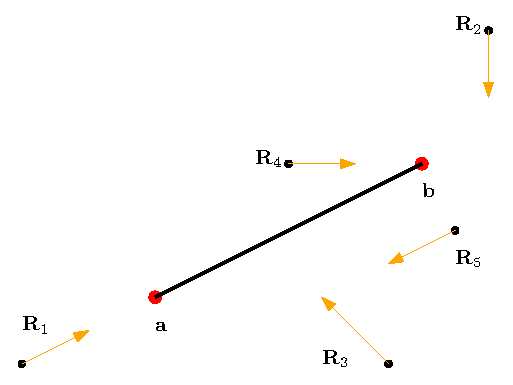
\includegraphics[width=0.50\textwidth]{img/segment2rays}
  \caption{Diferents rays $\mathbf{R}_i$ and their test of intersection with segment $\overline{\mathbf{a}\mathbf{b}}$}
  \label{fig:rays2seg}
\end{figure}

The Figure~\ref{fig:rays2seg} shows the different cases: 
\begin{itemize}
  \item $\mathbf{R}_1$ Hits the whole segment. In fact, both reside on the same line. This is a hit.
  \item $\mathbf{R}_2$ does not the segment.
  \item $\mathbf{R}_3$ hits the segment in the middle.
  \item $\mathbf{R}_4$ kisses (touches) the segmnet at his endpoint. By convention we say this is a hit.
  \item $\mathbf{R}_5$ is parrallel to the segment but does not touch it.
  \item $\mathbf{R}_6$ is parrallel to the segment, is on the same line, but also does not touch it.
\end{itemize}

In the scenario described above, the ray is $\mathbf{R}(s) = \mathbf{o} + s \mathbf{v}$ with $s \geq 0$ and the segment is $\mathbf{S}(t) = \mathbf{a} + t (\mathbf{b} - \mathbf{a})$ with $0 \leq t \leq 1$.
If $\mathbf{R}(s)$ intersects $\overline{\mathbf{a}\mathbf{b}}$, then $\mathbf{R}(s) = \mathbf{S}(t)$ for some values of $\mathbf{s}$ and $\mathbf{t}$.

\begin{align*}
\mathbf{a} + t (\mathbf{b} - \mathbf{a}) &= \mathbf{o} + s \mathbf{v} \\
\mathbf{a} - \mathbf{o} &= s \mathbf{v} + t (\mathbf{a} - \mathbf{b}) \\
\begin{bmatrix}
\mathbf{a} - \mathbf{o}  \\
 ~ 
\end{bmatrix} &= 
\begin{bmatrix}
\mathbf{v} & \mathbf{a} - \mathbf{b} \\
~ & ~
\end{bmatrix}
\begin{bmatrix}
s \\
t 
\end{bmatrix} \\
\begin{bmatrix}
a_x - o_x  \\
a_y - o_y
\end{bmatrix} &= 
\begin{bmatrix}
v_x & a_x - b_x \\
v_y & a_y - b_y
\end{bmatrix}
\begin{bmatrix}
s \\
t 
\end{bmatrix}
\end{align*}

Which is a $2 \times 2$ linear equations system that we can solve to get the values of $s$ and $t$.
We will solve it by Cramer's rule. 
Therefore, first we define:
\begin{align*}
\Delta =&  
\begin{vmatrix}
v_x & a_x - b_x \\
v_y & a_y - b_y
\end{vmatrix} \\
\Delta_s =&  
\begin{vmatrix}
a_x - o_x & a_x - b_x \\
a_y - o_y & a_y - b_y
\end{vmatrix} \\
\Delta_t =&  
\begin{vmatrix}
v_x & a_x - o_x \\
v_y & a_y - o_y
\end{vmatrix} \\
\end{align*}

An interesting observation, is that if we identify the previous determinats with the equations of the ray and the segement; 
we see that $\Delta$ is  concerned with the linear independence of the directional vectors $\mathbf{v}$ and $\mathbf{a} - \mathbf{b}$.
Meanwhile, $\Delta_s$ and $\Delta_t$ are concerned with the linear independence of each of the directional vectors with $\mathbf{a} - \mathbf{o}$ which is the diference between both origin ($\mathbf{a}$ is in a sense the origin of $\mathbf{S}$) points.

In other words if $\Delta = 0$ then, the directional vectors are parallel.
If $\Delta_s =  0$ or $\Delta_t = 0$ then, $\mathbf{a} - \mathbf{o}$ is parrallel with one of the directional vectors.

Finally, we get values for $s$ and $t$ by:

\begin{align*}
s = \frac{\Delta_s}{\Delta} =&  \frac{(a_x - o_x)(a_y - b_y) - (a_y - o_y)(a_x - b_x)}{v_x(a_y - b_y) - v_y(a_x - b_x)} \\
t = \frac{\Delta_t}{\Delta} =&  \frac{v_x(a_y - o_y) - v_y(a_x - o_x)}{v_x(a_y - b_y) - v_y(a_x - b_x)}
\end{align*}

Lets assume that the system has a unique soution: $\Delta \neq 0$. We can check the values $s$ and $t$. If both of the values fall in the desired range then, $\mathbf{R}$ intersects $\mathbf{S}$. If at least one of the values is ouside the range, $\mathbf{R}$ does not intersects $\mathbf{S}$.

When $\Delta = 0$ means that we have linear dependency of the vectors $\mathbf{v}$ and $\mathbf{a} - \mathbf{b}$ (or $\mathbf{b} - \mathbf{a}$ if that matters).
If we look again at Figure~\ref{fig:rays2seg} this means that the ray and the segment are parallel.
There is again two possible geometric situations for this. One of them also divides in sub cases.
In summary, if $\Delta = 0$ we have any of the following situations for $\mathbf{R}$ and $\mathbf{S}$:
\begin{enumerate}
  \item They do not reside on the same line. Like the case of $\mathbf{R}_5$ in the Figure~\ref{fig:rays2seg}.
  \item They reside on the same line. Then, we have two possible subcases:
  \begin{enumerate}
    \item They do not intersect: $\mathbf{R}$ is not inside $\overline{\mathbf{a}\mathbf{b}}$ and shoots away from it. This is the situation for $\mathbf{R}_6$ in the Figure~\ref{fig:rays2seg}.
    \item They do intersect. In fact, they overlap. $\mathbf{R}$ is either on $\overline{\mathbf{a}\mathbf{b}}$ or shooting into it. This is the situation for $\mathbf{R}_1$ in the Figure~\ref{fig:rays2seg}.
  \end{enumerate}
\end{enumerate}

All the above led us to Algorithm~\ref{alg:ray2seg}:

{\centering
\begin{minipage}{\linewidth}
  \begin{algorithm}[H]
    \caption{Intersection test between a ray $\mathbf{R}$ and a line segment $\overline{\mathbf{a}\mathbf{b})}$}
    \label{alg:ray2seg}
    \begin{algorithmic}[1] % The number tells where the line numbering should start 0 for no number
      \Procedure{RayIntersectSegment}{$\mathbf{a},\mathbf{b},\mathbf{o},\mathbf{v}$} \Comment{$\mathbf{a}, \mathbf{b}, \mathbf{o} \in \mathbb{R}^2$ are all points. $\mathbf{v} \in \mathbb{R}^2$ it's the direction vector of the ray}
      \If{$|\mathbf{v}|^2 = 0$} \Comment{There is no ray}
          \State \Return{false}
      \EndIf
      \If{$\mathbf{a} = \mathbf{b}$} \Comment{The segment it's just a point}
          \State \Return{\Call{RayHitsPoint}{$\mathbf{o},\mathbf{v},\mathbf{a}$}}
      \EndIf
      \State $\Delta \gets v_x(a_y - b_y) - v_y(a_x - b_x)$
      \State $\Delta_s \gets (a_x - o_x)(a_y - b_y) - (a_y - o_y)(a_x - b_x)$
      \State $\Delta_t \gets v_x(a_y - o_y) - v_y(a_x - o_x)$
      \If{$\Delta \neq 0$} \Comment{Ray and segment are not parralell. Perform normal test}
          \State $s \gets \Delta_s / \Delta$
          \State $t \gets \Delta_t / \Delta$
          \If{$0 \leq t \leq 1$ \textbf{and} $s \geq 0$} \Comment{They intersect}
            \State \Return{true}
          \Else \Comment{They do not intersect}
            \State \Return{false}
          \EndIf
      \EndIf
      \If{$\Delta_s \neq 0$} \Comment{They are parallel but they are not in the same line}
        \State \Return{false}
      \EndIf
      \State $s_p \gets \frac{(\mathbf{o} - \mathbf{a}) \cdot (\mathbf{b} - \mathbf{a})}{|\mathbf{b} - \mathbf{a}|^2}$ \Comment{They are on the same line. Check relative positions of $\mathbf{o}$ and $\overline{\mathbf{a}\mathbf{b}}$}
      \State \Return{$s_p \leq 1$}
      \EndProcedure
      \State
      \Procedure{RayHitsPoint}{$\mathbf{o},\mathbf{v},\mathbf{p}$} \Comment{$\mathbf{o}, \mathbf{p} \in \mathbb{R}^2$ are points. $\mathbf{v} \in \mathbb{R}^2$ it's the direction vector of the ray}
        \If{$|\mathbf{v}|^2 = 0$} \Comment{There is no ray}
          \State \Return{false}
        \EndIf
        \State $s_q \gets \frac{(\mathbf{p} - \mathbf{o}) \cdot \mathbf{v}}{|\mathbf{v}|^2}$
        \If{$s_q < 0$} \Comment{The point is behind the ray}
           \State \Return{false}
        \EndIf
        \State $\mathbf{q} \gets \mathbf{o} + s_q \mathbf{v}$ \Comment{Project the point into the ray}
        \State \Return{$\mathbf{q} = \mathbf{a}$} \Comment{Test if the point was on the ray}
      \EndProcedure
    \end{algorithmic}
  \end{algorithm}
\end{minipage}
\par
}

{\centering
\begin{minipage}{\linewidth}
  \begin{listing}[H]
  \inputminted[
  xleftmargin=1.5cm,  %without this option line number goes wrong
  %frame=lines,
  framesep=0.5cm,
  baselinestretch=1.2,
  fontsize=\footnotesize,
  linenos,
  firstline=78, %If you omit this two fields, the whole file is pulled
  lastline=123
  ]{cpp}{src/testAnaGeo.cpp}
  \caption{Implementation of Algorthm~\ref{alg:ray2seg} in C++ and GLM}
  \label{lst:ray2seg}
  \end{listing}
\end{minipage}
\par
}

\subsection{Belonging test on simple polygons}
\label{sec:belongTest}

In principle, this problem does not seem to be related to the previos ones.
However, the algorithm to solve it does really on all the previos algorithms.

As it is ussual in CG, we represent a simple polygon\footnote{A \emph{simple} polygon is one in which his edges only intersect in their respective endpoints} $\mathbf{P}$ with an ordered list $V$, $|V| \geq 3$ of points in $\mathbb{R}^2$ that represent his consecutive vertices.
By convention, we assume that there is an extra edge between the first and last point in $V$.

Now, if we have an extra point $\mathbf{p} \in \mathbb{R}^2$.
The problem is to determine if $\mathbf{p}$ it's in the interior region of $\mathbf{P}$.
\footnote{By \href{https://en.wikipedia.org/wiki/Jordan_curve_theorem}{Jordan's curve theorem}, any simple polygon will divide $\mathbb{R}^2$ in three regions: his interior, his exterior and his boundary. In our case, by convention; we will consider the boundary to be part of the interior.}

Since we know, thanks to the \href{https://en.wikipedia.org/wiki/Jordan_curve_theorem}{Jordan's curve theorem} that any path that connects the interioir with the exterior will need to cross the boundary.
That the boundary is $\mathbf{P}$.
And that all the points in $V$ are finite. 
Therefore, we can generate a very simple and elegant algorithm to solve our problem.

Shoot any ray $\mathbf{R}$ from $\mathbf{p}$, then count how many of the segments defined by $L$ are intersected by $\mathbf{R}$. 
If the number of intersections is even, then $\mathbf{p}$ was in the exterior of $\mathbf{P}$, else (i.e the number of intersections is odd) $\mathbf{p}$ is in the interior of $\mathbf{P}$.\footnote{Remember, that zero it's an even number. So, no intersection means that $\mathbf{p}$ was in the exterior of $\mathbf{P}$}

In principle \emph{any} ray $\mathbf{R}$ will work.
However, due numerical stabillity and to simplify a lot of calculations; we use an horizontal ray shooted to the right of $\mathbf{p}$

The Figure~\ref{fig:polygonTest} shows a simple polygon and several points $\mathbf{p}_i$.
The different points $\mathbf{p}_i$ are shown in black, each of them spawn a corresponding ray $\mathbf{R}_i$, shown in a dashed orange line.
The polygon $\mathbf{P}$ it's defined by his vertices $V$ shown in red.
We can see that $\mathbf{R}_1$ and $\mathbf{R}_5$ hit the poligon edges an odd number of times, therefore they are inside of $\mathbf{P}$.
In contrast, $\mathbf{R}_2$ and $\mathbf{R}_4$ hit an even number of times and they are outside of $\mathbf{P}$
It also shows an interesting corner case: $\mathbf{R}_3$, (How many times does $\mathbf{R}_3$ crosses the boundary?) that we will discuss below.

\begin{figure}[htb]
  \centering
  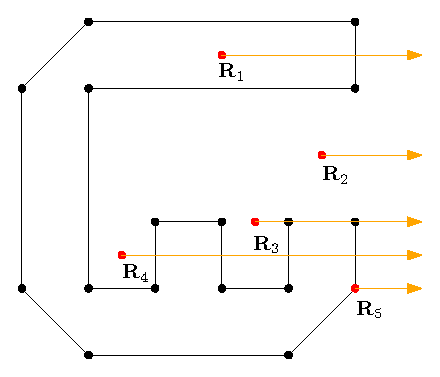
\includegraphics[width=0.50\textwidth]{img/polygonTest}
  \caption{Diferents points $\mathbf{p}_i$ and their test of belonging to a polygon}
  \label{fig:polygonTest}
\end{figure}

By convention if a point its exactlly on any of the edges of $\mathbf{P}$ (like $\mathbf{p}_5$), we will say it belongs to the polygon.


